\documentclass{amsart}
\usepackage{graphicx}
\graphicspath{{./}}
\usepackage{hyperref}
\usepackage{csvsimple}
\usepackage{longtable}
\usepackage{epigraph}
\title{Ethnicity and Support for Political Violence and Terrorism}
\author{Zulfikar Moinuddin Ahmed}
\date{\today}
\begin{document}
\maketitle

\section{Angels are quite interested in All Manner of Virtues of Human Race}

We are Angels.  We are most interested in accurate assessment of whether Human Race is Angelic or not.  If you are Angelic, good.  If not we might end up having to take action against Human Race, which may include simply totally wiping all Human Race from Existence.  We have headaches if you are not Angelic.  You might become a Demonic Civilisation and put a number of Angelic Worlds under threat.  We hate it when potential Angelic Civilisations become the hub of Demonic threats to large number of Angelic Worlds.  Demons love to take secret bases.

\section{Back to Earth}

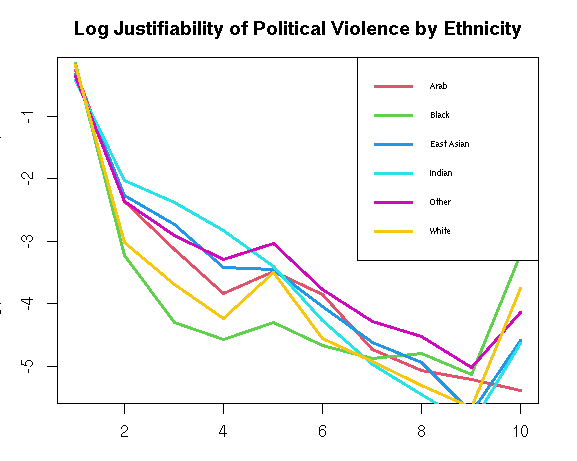
\includegraphics[scale=0.8]{ethterror.jpeg}

As I suspected, white people and Indians like me are much more likely to be enthusiastic about political violence than Arabs.  Most interesting indeed.
 
We can look at the actual distribution of support from 1=Never to 10=Always without taking a log.

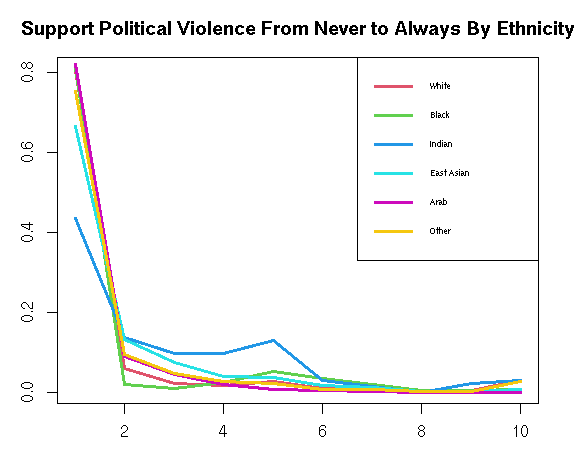
\includegraphics[scale=0.8]{pveth.jpeg}

This tells us immediately that the mass of people believe political violence is never justified.

Let us get a quantitative grasp of the situation by looking carefully at the tail mass say 6-10 for each ethnicity.  I like to look at this because I feel that since 9/11 there has been an enormous amount of disinformation and ethnic-propaganda and most of it is wrong.  Let us set this straight since we have high quality data here from World Values Survey Wave 7.

% latex table generated in R 4.0.3 by xtable 1.8-4 package
% Sat May  1 19:43:29 2021
\begin{table}[ht]
\centering
\begin{tabular}{rlr}
  \hline
 & eth & tail \\ 
  \hline
1 & White & 0.06 \\ 
  2 & Black & 0.08 \\ 
  3 & Indian & 0.10 \\ 
  4 & East Asian & 0.05 \\ 
  5 & Arab & 0.01 \\ 
  6 & Other & 0.05 \\ 
   \hline
\end{tabular}
\end{table}

Most intriguing.  The most prominent feature here is that Arabs are actually the least enthusiastic about terrorism.

Let's look even further to the extreme, now levels 8-10.

% latex table generated in R 4.0.3 by xtable 1.8-4 package
% Sat May  1 19:45:56 2021
\begin{table}[ht]
\centering
\begin{tabular}{rlr}
  \hline
 & eth & tail \\ 
  \hline
1 & White & 0.04 \\ 
  2 & Black & 0.02 \\ 
  3 & Indian & 0.05 \\ 
  4 & East Asian & 0.02 \\ 
  5 & Arab & 0.00 \\ 
  6 & Other & 0.03 \\ 
   \hline
\end{tabular}
\end{table}

This shows how the justification for terrorism is subtle, for now we lose blacks.  There are simply no Arabs in the estimate here.  Finally, the most extreme tail level 10.

% latex table generated in R 4.0.3 by xtable 1.8-4 package
% Sat May  1 19:48:53 2021
\begin{table}[ht]
\centering
\begin{tabular}{rlr}
  \hline
 & eth & tail \\ 
  \hline
1 & White & 0.03 \\ 
  2 & Black & 0.01 \\ 
  3 & Indian & 0.03 \\ 
  4 & East Asian & 0.01 \\ 
  5 & Arab & 0.00 \\ 
  6 & Other & 0.03 \\ 
   \hline
\end{tabular}
\end{table}

This is most intriguing: only whites and Indians have views for political violence always justified at around 3\% level.

\section{Deeper Examination}

The white $\lambda$ parameter is $\lambda_{white} = 0.3407$ which gives tail probability
\[
P_{\ge 10} = 0.033
\]
It is not a fair comparison with Indian version because the Indian curve fit to exponential is not as good as white, and $\lambda_{indian} = 0.6124$ which would give a much smaller tail probability for Indian using exponential model fit.  

\section{Substantial Conclusion}

Based purely on World Value Survey Analysis, we would conclude that tail of support for political violence ought to consider whites and indians as candidates for consideration for political extremism much more than blacks, Arabs, East Asians.
 
\section{Recommendation against Wiping Out Human Race}

These data show that Human Race is overall strongly against political violence across major ethnicities, and are therefore Angelic.  We see some minor tail populations of Indians and White people who are a bit enthusiastic about political violence but these are most likely minor.  Zulf recommends some patience.  I like this Race and I don't like Races I like being wiped out by Angels generally.  I will support no wiping out Human Race.  The Race looks quite promising and we ought to employ Patience.

\end{document}
\maketitle

\end{document}
